\newpage
\subsection{WiFi verbinding}
\subsubsection{Klassendiagram}
Om de verzamelde informatie te versturen wordt er gebruik gemaakt van een WiFi verbinding die aangemaakt wordt wanneer de SenseBox opstart. Dit is ook een singleton omdat er maar één wifi antenne is en er dus maar met één netwerk tegelijk verbinding gemaakt kan worden. Het ip address wordt opgeslagen in de klasse zodat deze later opgevraagd kan worden buiten de klasse. Bij het aanmaken van een WiFi verbinding moeten de inloggegevens voor het netwerk meegegeven worden in de constructor.

\begin{figure}[H]
  \centering
  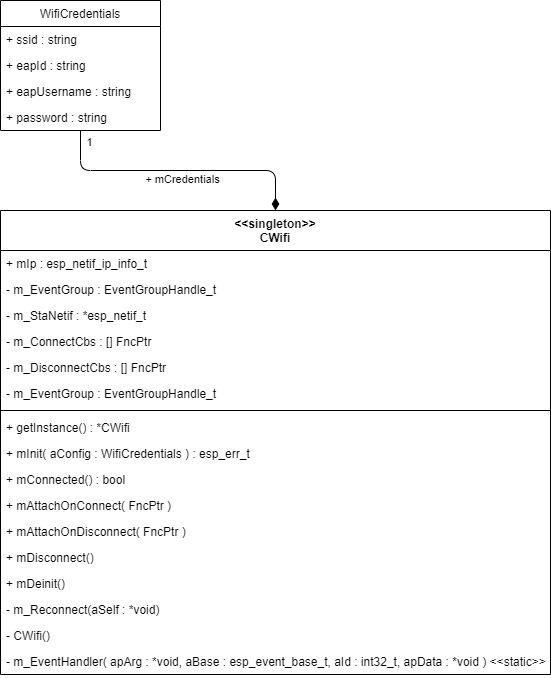
\includegraphics[width=.6\columnwidth]{uml/wifi-network-stack.png}
\end{figure}

\newpage
\subsubsection{Toestandsdiagram}
Wanneer de WiFi verbinding gestart wordt moeten de inloggegevens meegegeven worden met de constructor. Als de EAP gebruikersnaam hierin niet leeg is weten we dat we met een WPA2 Enterprise netwerk willen verbinden, dit is nodig om met het netwerk op school te kunnen verbinden. Als de gebruikersnaam leeg is moet er verbonden worden met een normaal WPA2 netwerk zoals je dat thuis hebt. Vanuit de WiFi verbinding kunnen er verschillende events gegenereerd worden die opgevangen moeten worden door de \emph{m\_EventHandler} member functie. Als dit gebeurt wordt de status van de verbinding bijgewerkt.
\vspace{1em}
Omdat er gebruik gemaakt wordt van FreeRTOS kunnen andere functies van FreeRTOS direct gebruik maken van de WiFi verbinding zonder dat hiervoor een speciale write of read functie aangemaakt moet worden. Dit is dan ook niet opgenomen in de toestandsdiagram.

\begin{figure}[H]
  \centering
  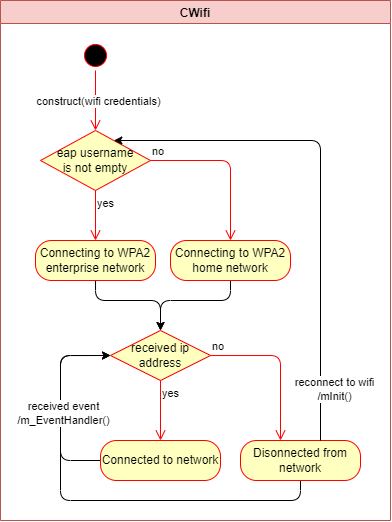
\includegraphics[width=.45\columnwidth]{uml/wifi-state-diagram.png}
\end{figure}